\documentclass[12pt]{book}

\usepackage[paperwidth=4.5in, paperheight=7in]{geometry}
\usepackage{graphicx}
\usepackage{parskip}
\usepackage{titlesec}
\usepackage{color}
\usepackage{subcaption}
\usepackage{needspace}

\definecolor{on}{RGB}{28, 113, 17}
\definecolor{off}{RGB}{233, 19, 19}
\definecolor{unknown}{RGB}{67, 107, 204}

\frenchspacing

\newcommand{\ON}{\textcolor{on}{ON}}
\newcommand{\OFF}{\textcolor{off}{OFF}}

\titleformat{\chapter}[display]{\normalfont\huge\bfseries}{}{0pt}{\Huge}\titlespacing*{\chapter}{0pt}{-50pt}{20pt}

\title{\includegraphics[width=\textwidth]{GameLogo}}
\author{Vincent Macri \and Chloe Nguyen \and Susie Son}
\date{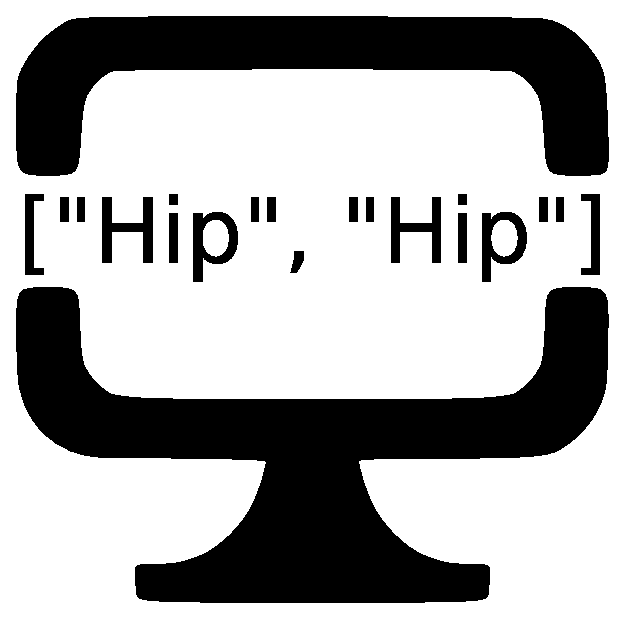
\includegraphics[width=0.5\textwidth]{CompanyLogo}\\\copyright 2017 Hip Hip Array}

\begin{document}
	\pagenumbering{gobble}
	\maketitle
	\begingroup
		\frontmatter
		\let\cleardoublepage\clearpage
		\tableofcontents
		\mainmatter
	\endgroup
	\chapter{The Story}
		You are the world's best ICS teacher, Ms. Krasteva. As a thank you gift for an amazing year of teaching, your students bought you a coffee. But when you drink the coffee, you start to feel funny.

		When you get home, you turn on your TV, and start to watch the news. They are running a story on a coffee recall! Due to horrible quality control, coffee from Starbucks is turning people sick. But not just a normal kind of sick. It is turning them into mice!

		You see the world around you getting bigger, but it isn't. Ms. Krasteva is turning into Mouse Krasteva!

		The news wrapped up the story by mentioning that the company ``Hip Hip Array'' is testing an antidote. However, you do not have time to wait for this antidote, because you need to mark the fantastic ISPs your students have poured the last month of their lives into in an effort to get 100%.

		You take it upon yourself to break into the lab and steal the antidote because mice are unable to use computer mice.

		Unfortunately for you, the lab has a high-tech security system of boolean algebra mazes and cat security guards, meaning that you have to avoid getting electrocuted while collecting fish to bribe the cats to not to eat you.
		\begin{center}
			\includegraphics[width=0.4\textwidth]{Cat}
			\hspace{5mm}
			\includegraphics[width=0.4\textwidth]{Mouse}
		\end{center}
		
	\chapter{Main Menu}
		The menu provides you with a few options:
		\begin{description}
			\item[New Game]
			\item[Continue]
			\item[Tutorial]
			\item[Settings]
			\item[High Scores]
			\item[Quit]
		\end{description}
		\newpage
		\begin{center}
			\vspace{2cm}
			\Huge
			Screenshot here		
		\end{center}
	\chapter{Settings}
		\begin{center}
			\vspace{2cm}
			\Huge
			Screenshot here		
		\end{center}
		On the settings menu, you are able to:
		\begin{itemize}
			\item Adjust the volume level
			\item Toggle fullscreen mode
			\item Change the controls
			\item Reset the settings, save, or everything
		\end{itemize}
	\chapter{Maze}
		In the maze, you must navigate through logic gates.

		Each gate has two inputs, and one output.
		\\
		\textcolor{on}{Green is on, or true.}
		\\
		\textcolor{off}{Red is off, or false.}
		\\
		\textcolor{unknown}{Blue is unknown.}

		\begin{figure}[h]
			\centering
			\begin{subfigure}[t]{0.3\textwidth}
				\centering
				\includegraphics[width=0.3\textwidth]{ON}

				An on wire.
			\end{subfigure}
			\hspace{1mm}
			\begin{subfigure}[t]{0.3\textwidth}
				\centering
				\includegraphics[width=0.3\textwidth]{OFF}

				An off wire.
			\end{subfigure}
			\hspace{1mm}
			\begin{subfigure}[t]{0.3\textwidth}
				\centering
				\includegraphics[width=0.3\textwidth]{UNKNOWN}

				An unknown wire.
			\end{subfigure}
		\end{figure}

		The two inputs will always be known, and \emph{you} will always need to determine the output.

		You will be working with AND, NAND, OR, NOR, and XOR gates.
		\section{AND Gate}
			An AND gate is on only if both of its inputs are on.
			\begin{center}
				\begin{tabular}{|c|c|c|}
					\hline
					\textbf{Input A} & \textbf{Input B} & \textbf{Output}\\\hline
					\OFF & \OFF & \OFF\\\hline
					\OFF & \ON & \OFF\\\hline
					\ON & \OFF & \OFF\\\hline
					\ON & \ON & \ON\\\hline
				\end{tabular}
			\end{center}
		\section{NAND Gate}
			A NAND gate's output is the opposite of an AND gate's with the same inputs. It is a \emph{not} AND gate.
			\begin{center}
				\begin{tabular}{|c|c|c|}
					\hline
					\textbf{Input A} & \textbf{Input B} & \textbf{Output}\\\hline
					\OFF & \OFF & \ON\\\hline
					\OFF & \ON & \ON\\\hline
					\ON & \OFF & \ON\\\hline
					\ON & \ON & \OFF\\\hline
				\end{tabular}
			\end{center}
		\section{OR Gate}
			An OR gate is on if at least of its inputs are on.
			\begin{center}
				\begin{tabular}{|c|c|c|}
					\hline
					\textbf{Input A} & \textbf{Input B} & \textbf{Output}\\\hline
					\OFF & \OFF & \OFF\\\hline
					\OFF & \ON & \ON\\\hline
					\ON & \OFF & \ON\\\hline
					\ON & \ON & \ON\\\hline
				\end{tabular}
			\end{center}
		\section{NOR Gate}
			A NOR gate's output is the opposite of an OR gate's with the same inputs. It is a \emph{not} OR gate.
			\begin{center}
				\begin{tabular}{|c|c|c|}
					\hline
					\textbf{Input A} & \textbf{Input B} & \textbf{Output}\\\hline
					\OFF & \OFF & \ON\\\hline
					\OFF & \ON & \OFF\\\hline
					\ON & \OFF & \OFF\\\hline
					\ON & \ON & \OFF\\\hline
				\end{tabular}
			\end{center}
		\section{XOR Gate}
			An XOR gate is on if only one of its inputs are on.
			\begin{center}
				\begin{tabular}{|c|c|c|}
					\hline
					\textbf{Input A} & \textbf{Input B} & \textbf{Output}\\\hline
					\OFF & \OFF & \OFF\\\hline
					\OFF & \ON & \ON\\\hline
					\ON & \OFF & \ON\\\hline
					\ON & \ON & \OFF\\\hline
				\end{tabular}
			\end{center}
		\section{Interacting with Gates}
			The goal of this game is to reach the right side of the map without touching any wires that are on. While not necessary, you make click on the gates to mark them with what you think their output is. Left click a gate to mark it as on. Right click a gate to mark it as off. Middle click a gate to mark it as unknown.
\end{document}
